\section{Verification and numerical resolution}
\label{sec:verification}

Verification uses analytical limiting cases, transfer-matrix relations, matrix identities and mesh refinement. The published heterogeneous-bilayer comparisons are more limited: source curves are available only as plots, and some parameter conventions are unclear. We do not use those comparisons as quantitative validation.

\subsection{Analytical limits and bilayer comparison}
In the isotropic homogeneous limit, the long-wavelength phase velocities recover the classical transverse and longitudinal speeds:
\begin{equation}
\begin{split}
\lim_{k\to0}\frac{\omega_T(k)}{k}&=\sqrt{\frac{\mu}{\rho}}=1.0,\\
\lim_{k\to0}\frac{\omega_L(k)}{k}&=\sqrt{\frac{\lambda+2\mu}{\rho}}=\sqrt{3}\approx1.73205.
\end{split}
\label{eq:acoustic_limits}
\end{equation}
At $\bar{k}=0.001$, the computed acoustic speeds differ from these limits by $1.25\times10^{-8}$ (Table~\ref{tab:consistency_suite}). The pure-bending micro-beam reduction matches the published closed-form limits within $10^{-15}$ \cite{papargyribeskou2009}. The micro-inertia asymptote is checked against the analytical result in Appendix~\ref{app:asymptotics}.

As a classical reference, we analyze a periodic AlN/BaTiO$_3$ bilayer with $a_A=a_B=0.01\,\mathrm{m}$ and $b=a_A+a_B=0.02\,\mathrm{m}$ using the Rytov relation \cite{li2024anchorB,zhengwei2009}:
\begin{equation}
\begin{split}
\cos(Kb)={}&\cos(k_Aa_A)\cos(k_Ba_B) \\
&-\frac{1}{2}\left(\frac{Z_A}{Z_B}+\frac{Z_B}{Z_A}\right)\sin(k_Aa_A)\sin(k_Ba_B),
\end{split}
\label{eq:rytov}
\end{equation}
where $k_m=\omega\sqrt{\rho_m/c_{33,m}}$, $v_m=\sqrt{c_{33,m}/\rho_m}$, and $Z_m=\rho_m v_m$. The single-layer transfer-matrix identity and the identical-material bilayer reduction match their analytical limits to $6.47\times10^{-16}$ and $7.22\times10^{-16}$, respectively. The heterogeneous transfer-matrix trace reproduces the Rytov relation to $2.22\times10^{-16}$. The first three calculated stop-band intervals are $[0.4806,0.5209]$, $[0.9812,1.0215]$, and $[1.4993,1.5028]$ in normalized frequency. We compare the result with the published B1 plot visually because tabulated source data are unavailable; no percentage error is inferred from the curves.

We reproduce two gradient-elastic bilayer cases, but do not treat them as external validations. One published length-scale definition is dimensionally ambiguous. For the other, the plotted parameter set and normalization are unspecified, and the numerical curves are unavailable. The parameter interpretations and limitations are documented in Appendix~\ref{app:transfer_checks}. Reproducing the printed dipolar layer matrix checks its algebra, not the published band curves.

\subsection{Numerical consistency and mesh convergence}
Table~\ref{tab:consistency_suite} reports eight checks covering matrix properties, reciprocal-space periodicity, rotational symmetry, acoustic limits, micro-inertia and energy transport. For the energy-flux check, we use closed-form Case-H harmonic fields and the sign convention in Appendix~\ref{app:energy_flux}. The flux-derived velocity agrees with the central-difference group velocity to $6.91\times10^{-10}$ across the tested directions and acoustic branches. The supporting numerical diagnostics are reported in Appendix~\ref{app:numerical_checks}.

Mesh convergence is tested in homogeneous Case~H at $\bmk=(0.31\pi/L,0.22\pi/L)$ using BFS grids with $n=4,8,16$ and $32$ elements per side. Figure~\ref{fig:mesh_convergence} shows the acoustic-frequency error relative to the closed-form value and the change between successive meshes. The first three mesh levels give an empirical rate of $p=4.17$ (95\% CI $[3.15,5.20]$). The $32^2$ result is close to the numerical resolution limit and was omitted from the fit. The fitted rate is not presented as a theoretical convergence order. The measured floor for successive-mesh changes is $\varepsilon_\Delta=4.63\times10^{-11}$; it should not be confused with eigensolver reproducibility. The smallest positive sampled directional separation across the 42-configuration design map, $\Delta_{GX}=1.3\times10^{-3}$ (at $\mathrm{AR}=5$, $\theta=0^\circ$; see Table~\ref{tab:gap_summary}), exceeds the floor by approximately $3\times10^7$.

\begin{figure*}[htbp]
\centering
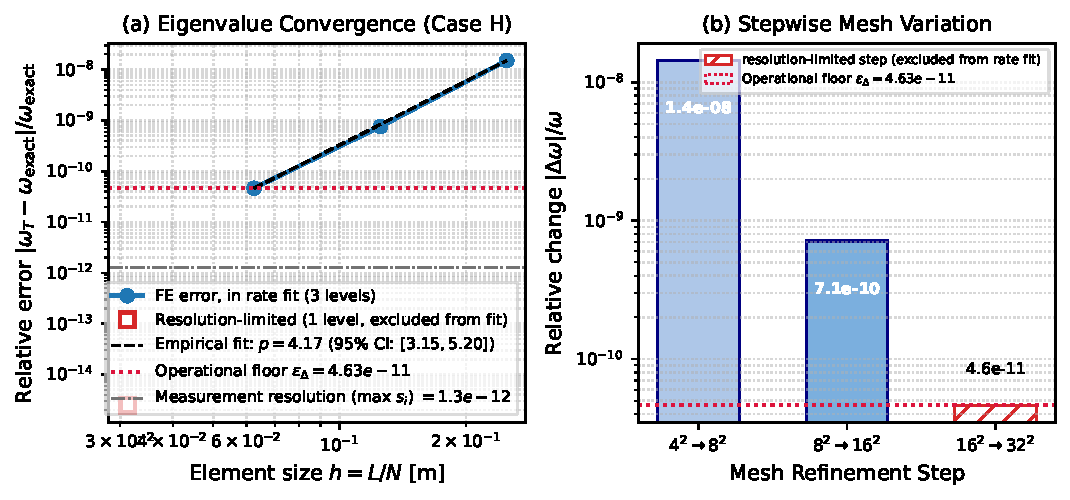
\includegraphics[width=\textwidth]{figures/fig05_mesh_convergence.pdf}
\caption{Case-H mesh convergence. (a) Acoustic-frequency error; the $32^2$ point is excluded from the empirical fit. (b) Successive-mesh changes and numerical floor $\varepsilon_\Delta$.}
\label{fig:mesh_convergence}
\end{figure*}

\begin{table*}[htbp]
\begin{center}
\begin{threeparttable}
\tablebodyfont
\caption{Numerical consistency checks. The energy-flux identity uses closed-form Case-H fields; other checks assess the Bloch finite-element implementation.}
\label{tab:consistency_suite}
\small
\begin{tabular}{@{}p{2.3cm} p{6.9cm} p{2.2cm} c p{1.8cm}@{}}
\toprule
Check & Quantity assessed & Maximum discrepancy & Criterion & Result \\
\midrule
Hermiticity & Reduced stiffness and mass operators & $2.01\times10^{-16}$; $5.63\times10^{-17}$ & $<10^{-12}$ & Within criterion \\
Brillouin-zone periodicity & Spectrum under reciprocal-lattice shifts & $9.66\times10^{-16}$ & $<10^{-10}$ & Within criterion \\
Isotropic rotation & Frequencies at $\mathrm{AR}=1$ & $9.63\times10^{-16}$ & $<10^{-10}$ & Within criterion \\
Acoustic limit & Long-wave transverse and longitudinal slopes & $1.25\times10^{-8}$ & $<10^{-6}$ & Within criterion \\
Rotation--swap symmetry & Spectrum under $\theta\mapsto\theta+90^\circ$ and axis swap & $6.44\times10^{-16}$ & $<10^{-10}$ & Within criterion \\
Definiteness & Two rigid modes at $\Gamma$; positive interior spectrum & As expected & Admissible & As expected \\
Micro-inertia limit & Phase speed at $\bar{k}=200$ versus asymptotic value & $2.85\times10^{-4}$ & $<10^{-3}$ & Within criterion \\
Energy-flux identity (closed-form) & Closed-form group velocity versus cycle-averaged energy flux, Case-H harmonic fields & $6.91\times10^{-10}$ & $<10^{-6}$ & Within criterion \\
\bottomrule
\end{tabular}

\end{threeparttable}
\end{center}
\end{table*}

Additional parameters and convergence data are tabulated in Appendix~\ref{app:extended_checks}.
